%\documentclass[handout]{beamer}
\documentclass[10pt]{beamer}
\usetheme[
  outer/progressbar=foot,
  outer/numbering=none
]{metropolis}
\usepackage{amsmath, amssymb, amsthm, mathtools,media9}
\usepackage[export]{adjustbox}

\usepackage[default]{sourcesanspro}
\usepackage[utf8]{inputenc}
\usepackage[T1]{fontenc}
\metroset{titleformat=smallcaps}

\usepackage{tikz}
\usetikzlibrary{mindmap,shadows}
\usepackage{animate}
\usepackage[compatibility=false]{caption}


\usepackage{graphicx,subfigure}
\usetikzlibrary{spy,calc,patterns,arrows,decorations.pathmorphing,backgrounds,positioning,fit,petri,mindmap,trees,intersections}
\usepackage{keystroke}
\usepackage{color}
\usepackage{multicol}
%\usepackage{multimedia}
\usepackage{enumerate}
\usepackage{multirow}
\usepackage{pgfplots,tikz,tcolorbox}
\usepackage{appendixnumberbeamer}



\pgfplotsset{compat=newest}
%\expandafter\def\expandafter\insertshorttitle\expandafter{%
 % \insertshorttitle\hfill\insertframenumber\,/\,\inserttotalframenumber}
%\usepackage{enumitem}


%\usepackage[T1]{fontenc}
\usepackage{color,hyperref}
\definecolor{darkblue}{rgb}{0.0,0.0,0.5}
%\hypersetup{colorlinks,breaklinks,
%            linkcolor=darkblue,urlcolor=darkblue,
%            anchorcolor=darkblue,citecolor=darkblue}
\usetikzlibrary{patterns}
\usetikzlibrary{decorations.pathmorphing,backgrounds,positioning,fit,petri,mindmap,trees}
\usepgflibrary{arrows,shapes.geometric}
\usepgflibrary{shapes.symbols}
%\hypersetup{colorlinks,breaklinks,linkcolor=darkblue,urlcolor=darkblue,anchorcolor=darkblue,citecolor=darkblue}
\usetikzlibrary{spy,calc,patterns,arrows,decorations.pathmorphing,backgrounds,positioning,fit,petri,mindmap,trees,intersections}
\usepackage{color}
\usepackage{multirow}
\usetikzlibrary{arrows,positioning} 
\tikzset{
    %Define standard arrow tip
    >=stealth',
    %Define style for boxes
    punkt/.style={
           rectangle,
           rounded corners,
           draw=black, very thick,
           text width=8.5em,
           minimum height=2em,
           text centered},
    % Define arrow style
    pil/.style={
           ->,
           thick,
           shorten <=2pt,
           shorten >=2pt,}
}

%\usepackage[hang]{footmisc}
%\setlength\footnotemargin{10pt}

\setbeamertemplate{caption}[numbered]
\usepgfplotslibrary{statistics}

\usetikzlibrary{fadings}
\tikzfading[name=fade out,
  inner color=transparent!0, outer color=transparent!100]


%\setbeameroption{show notes}


\newcommand{\network}[1]{
\begin{figure}[h]
\centering
\begin{tikzpicture}[scale = 0.75,-,draw=black!50, node distance=\layersep]
    \tikzstyle{neuron}=[circle,fill=black!25,minimum size=17pt,inner sep=0pt];
    \tikzstyle{unit}=[neuron, fill=red!50];
    \tikzstyle{spike}=[neuron, fill=blue!50];
 \def \radius {2cm}
% \def \margin {8}
 \def \n {6}
 \foreach \s in {1,...,\n}
  \node[unit] (\s) at ({360/\n * (\s - 1) - 180}:\radius) {$\s$};
 \foreach \s in {1,...,\n}
  \foreach \t in {\s,...,\n}
   \draw (\t) -- (\s);
 \foreach \s in {1,...,\n}
   \draw[very thick] (#1) -- (\s);
   \node[spike] (#1) at ({360/\n * (#1 - 1) - 180}:\radius) {};
\end{tikzpicture}
\end{figure}

}


\newcommand{\networkwc}[6]{
\begin{figure}[h]
\centering
\begin{tikzpicture}[scale = 1,-,draw=black!50, node distance=\layersep]
    \tikzstyle{neuron}=[circle,fill=black!25,minimum size=17pt,inner sep=0pt];
    \tikzstyle{unit}=[neuron, fill=red!50];
    \tikzstyle{spike}=[neuron, fill=blue!50];
 \def \radius {2cm}
% \def \margin {8}
 \def \n {6}
% \foreach \s in {1,...,\n}
  \node[unit] (1) at (- 180:\radius) {{\color{white}#1}};
   \node[unit] (2) at (- 120:\radius) {{\color{white}#2}};
     \node[unit] (3) at (- 60:\radius) {{\color{white}#3}};
   \node[unit] (4) at (0:\radius) {{\color{white}#4}};
  \node[unit] (5) at (60:\radius) {{\color{white}#5}};
   \node[unit] (6) at (120:\radius) {{\color{white}#6}};
 \foreach \s in {1,...,\n}
  \foreach \t in {\s,...,\n}
   \draw (\t) -- (\s);
% \foreach \s in {1,...,\n}
%   \draw[very thick] (#1) -- (\s);
%   \node[spike] (#1) at ({360/\n * (#1 - 1) - 180}:\radius) {};
\end{tikzpicture}
\end{figure}
}

\newcommand{\networkwcww}[6]{
\begin{figure}[h]
\centering
\begin{tikzpicture}[scale = 1,-,draw=black!50, node distance=\layersep]
    \tikzstyle{neuron}=[circle,fill=black!25,minimum size=17pt,inner sep=0pt];
    \tikzstyle{unit}=[neuron, fill=red!50];
    \tikzstyle{spike}=[neuron, fill=blue!50];
 \def \radius {2cm}
% \def \margin {8}
 \def \n {6}
% \foreach \s in {1,...,\n}
  \node[unit] (1) at (- 180:\radius) {{\color{white}#1}};
   \node[unit] (2) at (- 120:\radius) {{\color{white}#2}};
     \node[unit] (3) at (- 60:\radius) {{\color{white}#3}};
   \node[unit] (4) at (0:\radius) {{\color{white}#4}};
  \node[unit] (5) at (60:\radius) {{\color{white}#5}};
   \node[unit] (6) at (120:\radius) {{\color{white}#6}};
 \draw (1) edge node[below left] {\small $-1$} (2);
 \draw (2) edge node[below] {\small $-3$} (3);
  \draw (3) edge node[below right] {\small $-1$} (4);
   \draw (4) edge node[above right] {\small $3$} (5);
    \draw (5) edge node[above] {\small $-2$} (6);
         \draw (6) edge node[above left] {\small $3$} (1);
     \draw (2) edge node[right] {\small $2$} (6);
      \draw (3) edge node[left] {\small $3$} (5);
%  \draw (i) edge node[right] {\small $W_{ij} = W_{ji}$} (j);

 % \foreach \s in {1,...,\n}
%   \draw[very thick] (#1) -- (\s);
%   \node[spike] (#1) at ({360/\n * (#1 - 1) - 180}:\radius) {};
\end{tikzpicture}
\end{figure}
}

\newcommand{\mpm}[6]{
\begin{figure}[h]
\centering
\begin{tikzpicture}[scale = 1,-,draw=black!50, node distance=\layersep,>=stealth]
    \tikzstyle{neuron}=[circle,fill=black!25,minimum size=17pt,inner sep=0pt];
    \tikzstyle{unit}=[neuron, fill=red!50,thick];
 \def \radius {2cm}
% \def \margin {8}
 \def \n {6}
 \foreach \s in {1,...,\n}{
  \node[unit] (\s) at ({360/\n * (\s - 1) - 180}:\radius) {};
%  \node (S-\s) at ($(\s) + {360/\n * (\s - 1) - 180}:5mm$) {$s_i$};
}  

   \DoubleLine{1}{2}{<-,draw=black!50}{}{->,draw=black!50}{};
   \DoubleLine{1}{3}{<-,draw=black!50}{}{->,draw=black!50}{};
   \DoubleLine{1}{4}{<-,draw=black!50}{}{->,draw=black!50}{};
   \DoubleLine{1}{5}{<-,draw=black!50}{}{->,draw=black!50}{};
   \DoubleLine{1}{6}{<-,draw=black!50}{}{->,draw=black!50}{};
    \DoubleLine{2}{3}{<-,draw=black!50}{}{->,draw=black!50}{};
   \DoubleLine{2}{4}{<-,draw=black!50}{}{->,draw=black!50}{};
   \DoubleLine{2}{5}{<-,draw=black!50}{}{->,draw=black!50}{};
   \DoubleLine{2}{6}{<-,draw=black!50}{}{->,draw=black!50}{};
   \DoubleLine{3}{4}{<-,draw=black!50}{}{->,draw=black!50}{};
   \DoubleLine{3}{5}{<-,draw=black!50}{}{->,draw=black!50}{};
   \DoubleLine{3}{6}{<-,draw=black!50}{}{->,draw=black!50}{};
    \DoubleLine{4}{5}{<-,draw=black!50}{}{->,draw=black!50}{};
   \DoubleLine{4}{6}{<-,draw=black!50}{}{->,draw=black!50}{};
   \DoubleLine{5}{6}{<-,draw=black!50}{}{->,draw=black!50}{};

   \node[unit] (1) at (- 180:\radius) {{\color{white}#1}};
   \node[unit] (2) at (- 120:\radius) {{\color{white}#2}};
     \node[unit] (3) at (- 60:\radius) {{\color{white}#3}};
   \node[unit] (4) at (0:\radius) {{\color{white}#4}};
  \node[unit] (5) at (60:\radius) {{\color{white}#5}};
   \node[unit] (6) at (120:\radius) {{\color{white}#6}};
%   \draw[color=None] (i) edge node[right] {\small $W_{ij}$} (j);
%   \draw[color=None] (i) edge node[left] {\small $W_{ij}$} (j);
\end{tikzpicture}
\end{figure}

}

\newcommand\DoubleLine[7][1pt]{%
    \path(#2)--(#3)coordinate[at start](h1)coordinate[at end](h2);
    \draw[#4]($(h1)!#1!90:(h2)$)-- node [left=-.75mm] {#5} ($(h2)!#1!-90:(h1)$); 
    \draw[#6]($(h1)!#1!-90:(h2)$)-- node [right=-.75mm] {#7} ($(h2)!#1!90:(h1)$);
    }

\tikzstyle{innergrid}=[gray!80]
\tikzstyle{tile}=[green!60!black, thick]
\tikzstyle{sync}=[red!60!black, thick, dashed]
\tikzstyle{thread}=[->, decorate, decoration={snake, amplitude=.6}]
\tikzstyle{examplecell}=[fill=orange, opacity=.5]
\tikzstyle{kernelcall}=[#1, rounded corners=2pt, very thick, pattern color=#1]
\tikzstyle{kernelarrow}=[->, thick, out=90, in=180]
\tikzstyle{imglabel}=[anchor=west, text opacity=1.0, fill=white, fill opacity=.5,
                      text height=1ex, text depth=.25ex, rounded corners]

\newcommand\drawthread[4]{%
  \pgfmathsetmacro{\ybot}{(1 + \nrblockbodies) * #2}
  \draw [#1] (0.5, \ybot + 0.5 + #3) -- ++(#4 - 1, 0);%
}


\title{Simulating RNNs on GPUs}
\subtitle{Summer Project}
%\institute{SUTD}
\author{Zhangsheng Lai}
%\date{\today}

\pgfmathdeclarefunction{gauss}{2}{%
  \pgfmathparse{1/(#2*sqrt(2*pi))*exp(-((x-#1)^2)/(2*#2^2))}%
}
%\pgfmathdeclarefunction{gauss1}{2}{%
  %\pgfmathparse{(1/(#2*sqrt(2*pi))*exp(-((-x-#1)^2)/(2*#2^2)))*exp(-x)}%
%}
\pgfmathdeclarefunction{gauss2}{2}{%
  \pgfmathparse{(1/(#2*sqrt(2*pi))*exp(-0.5*abs(x)-#1)*(sqrt(abs(x)))}%
}

%\pgfmathdeclarefunction{gauss2}{2}{%
  %\pgfmathparse{(1/(#2*sqrt(2*pi))*exp(-((x-#1)^2)/(2*#2^2)))*exp(x)}%
%}
\pgfmathdeclarefunction{gauss1}{2}{%
  \pgfmathparse{(1/(#2*sqrt(2*pi))*exp(-0.5*x-#1)*(sqrt(x))}%
}
\def\checkmark{\tikz\fill[scale=0.4](0,.35) -- (.25,0) -- (1,.7) -- (.25,.15) -- cycle;}

\newcommand*{\Perm}[2]{{}^{#1}\!P_{#2}}%
\newcommand*{\Comb}[2]{{}^{#1}C_{#2}}%
\begin{document}


\begin{frame}
\titlepage
\end{frame}


%\begin{frame}
%\tableofcontents
%\end{frame}



\begin{frame}{Mult-layer Perceptron}
\begin{figure}[h]
\centering

\def\layersep{2cm}

\begin{tikzpicture}[scale = 1,draw=black!50, node distance=\layersep]
%    \tikzstyle{every pin edge}=[<-,shorten <=1pt]
    \tikzstyle{neuron}=[circle,fill=black!25,minimum size=10pt,inner sep=0pt]
    \tikzstyle{input neuron}=[neuron, fill=blue!70!red!70];
        \tikzstyle{hidden neuron 0}=[neuron, fill=blue!50!red!50];
    \tikzstyle{hidden neuron 1}=[neuron, fill=red!80];
    \tikzstyle{hidden neuron 2}=[neuron, fill=red!50];
        \tikzstyle{output neuron}=[neuron, fill=orange!70];

    \tikzstyle{annot} = [text width=4em, text centered]

    % Draw the input layer nodes
    \foreach \name / \y in {1,...,6}
    	\node[input neuron] (I-\name) at (0,-\y) {};
		\node[input neuron] (I-4) at (0,-4) {};

 \foreach \name / \y in {1,...,6}
    	            \node[hidden neuron 0] (B-\name) at (\layersep,-\y cm) {};


    % Draw the hidden layer nodes
    \foreach \name / \y in {1,...,6}
            \node[hidden neuron 1] (H-\name) at (2*\layersep,-\y cm) {};
    % Draw the output layer node
%    \node[output neuron,pin={[pin edge={->}]right:$h_{W,b}(x) = f(z_{1}^{(3)}) = a_{1}^{(3)}$}, right of=H-3] (O) {};
 \foreach \name / \y in {1,...,6}
            \node[hidden neuron 2] (P-\name) at (3*\layersep,-\y cm) {};

 \foreach \name / \y in {1,...,3}
 \path[yshift=-1.5cm]
      node[output neuron] (O-\name) at (4*\layersep,-\y cm) {};

    % Connect every node in the input layer with every node in the
    % hidden layer.
    \foreach \source in {1,...,6}
        \foreach \dest in {1,...,6}
            \path[color = blue!70!red!70] (I-\source) edge (B-\dest);

  \foreach \source in {1,...,6}
        \foreach \dest in {1,...,6}
            \path[color = blue!50!red!50] (B-\source) edge (H-\dest);

\foreach \source in {1,...,6}
        \foreach \dest in {1,...,6}
            \path[color = red!80] (H-\source) edge (P-\dest);

\foreach \source in {1,...,6}
        \foreach \dest in {1,...,3}
            \path[color = red!50] (P-\source) edge (O-\dest);

    \node[annot,below=0.25cm of {H-6}, node distance=1cm] (hl2) {\small {\color{red!80}L3}};
    \node[annot,left of=hl2](hl1) {\small {\color{blue!50!red!50}L2}};
        \node[annot,left of=hl1] {\small {\color{blue!70!red!70}L1}};
            \node[annot,right of=hl2](hl3) {\small {\color{red!50}L4}};
            \node[annot,right of=hl3] {\small {\color{orange!70}L5}};
\end{tikzpicture}
\caption{Multi-layer perceptron}
\label{fig:neural network}
\end{figure}
\end{frame}

\begin{frame}{}
\section{Hopfield Networks and Boltzmann Machines}
\end{frame}



\begin{frame}{Hopfield Networks}
\networkwc{1}{-1}{1}{1}{-1}{1}
\end{frame}

\begin{frame}{Hopfield Networks}
\networkwc{1}{0}{1}{1}{0}{1}
\end{frame}

\begin{frame}{Hopfield Networks}
\begin{figure}[h]
\centering
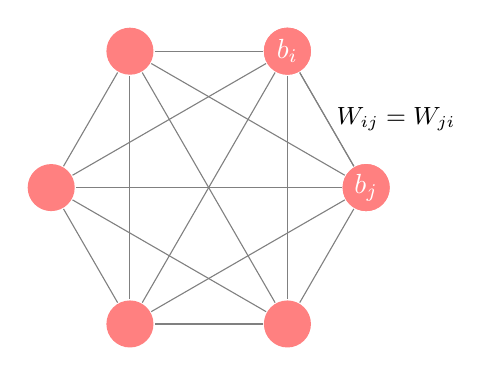
\begin{tikzpicture}[scale = 1,-,draw=black!50, node distance=\layersep]
    \tikzstyle{neuron}=[circle,fill=black!25,minimum size=17pt,inner sep=0pt];
    \tikzstyle{unit}=[neuron, fill=red!50,thick];
 \def \radius {2cm}
% \def \margin {8}
 \def \n {6}
 \foreach \s in {1,...,\n}{
  \node[unit] (\s) at ({360/\n * (\s - 1) - 180}:\radius) {};
%  \node (S-\s) at ($(\s) + {360/\n * (\s - 1) - 180}:5mm$) {$s_i$};
}  
 \foreach \s in {1,...,\n}
  \foreach \t in {\s,...,\n}
   \draw (\t) -- (\s);
   \node[unit](i) at ({60 }:\radius) {{\color{white}$b_i$}};
   \node[unit](j) at ({360}:\radius) {{\color{white}$b_j$}};
   \draw (i) edge node[right] {\small $W_{ij} = W_{ji}$} (j);

   \end{tikzpicture}
\end{figure}
\begin{align*}
\text{Energy configuration, }E &= -\sum_{i<j}W_{ij}x_ix_j - \sum_ib_i x_i \\
\text{Energy gap, } \Delta E_i &= E(x_i = 0) - E(x_i = 1) = \sum_jW_{ij}x_j +b_i\\
\text{Update rule, }x_i:&=\begin{cases}
+1 & \sum_jW_{ij}x_j +b_i \geq 0\\
-1 & \text{otherwise}
\end{cases}
\end{align*}
\end{frame}

\note{\scriptsize
\begin{itemize}
\item composed of primitive computing elements called units
\item units has two states, on or off, represented by $\{1,-1\}$ or $\{1,0\}$
\item connected to each other by bi-directional links
\item adopts these states as a function of the states of its neighbouring units and weights of its links to them, it is a probabilistic function for a Boltzmann machine.
\item weights can take on any real value
\item a unit being on or off is taken to mean that the system currently accepts or rejects some elemental hypothesis of the domain
\item weight on a link represents a weak pairwise constrain between two hypothesis
\item positive (negative) weights indicate that two hypothesis support (contradict) one another with other things being equal
\item link weights are symmetric, having the same strength in both directions
\end{itemize}
}


\begin{frame}{Hopfield Networks}
\networkwcww{1}{0}{0}{0}{0}{1}
\begin{align*}
(1,0,0,0,0,1)
\end{align*}
\end{frame}

\begin{frame}{Hopfield Networks}
\networkwcww{1}{1}{0}{0}{0}{1}
\begin{align*}
(1,0,0,0,0,1)\\
(1,1,0,0,0,1)
\end{align*}

\end{frame}

\begin{frame}{Hopfield Networks}
\networkwcww{0}{0}{1}{1}{1}{0}
\begin{align*}
(1,0,0,0,0,1)\\
(1,1,0,0,0,1)\\
(0,0,1,1,1,0)
\end{align*}

\end{frame}

\note{
\scriptsize
\begin{itemize}
\item Updating of Hopfield networks is done 	sequentially usually in a randomized order. Parallel updating might increase the energy instead.
%Asynchronous: one unit is updated at a time, can be done randomly or in a pre-defined order. Synchronous: all units are updated at the same time.
\item Hopfield networks always make decisions to reduce the energy and makes it impossible to escape from local minima.
\item random noise can help us escape from poor minima, by starting with lots of noise so its easy to cross energy barriers and gradually decrease the noise so the system ends in a deep minimum. This is called simulated annealing.
\end{itemize}
}


\begin{frame}{Boltzmann Machines}
\begin{figure}[h]
\centering
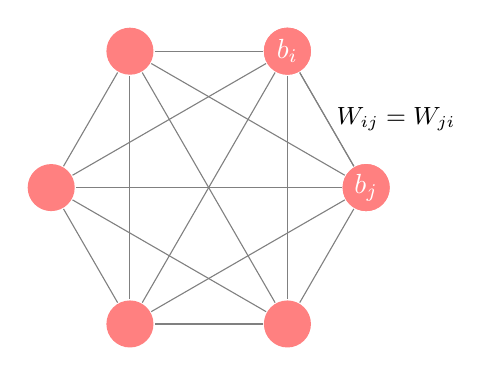
\begin{tikzpicture}[scale = 1,-,draw=black!50, node distance=\layersep]
    \tikzstyle{neuron}=[circle,fill=black!25,minimum size=17pt,inner sep=0pt];
    \tikzstyle{unit}=[neuron, fill=red!50,thick];
 \def \radius {2cm}
% \def \margin {8}
 \def \n {6}
 \foreach \s in {1,...,\n}{
  \node[unit] (\s) at ({360/\n * (\s - 1) - 180}:\radius) {};
%  \node (S-\s) at ($(\s) + {360/\n * (\s - 1) - 180}:5mm$) {$s_i$};
}  
 \foreach \s in {1,...,\n}
  \foreach \t in {\s,...,\n}
   \draw (\t) -- (\s);
   \node[unit](i) at ({60 }:\radius) {{\color{white}$b_i$}};
   \node[unit](j) at ({360}:\radius) {{\color{white}$b_j$}};
   \draw (i) edge node[right] {\small $W_{ij} = W_{ji}$} (j);

   \end{tikzpicture}
\end{figure}
\begin{align*}
E &= -\sum_{i<j}W_{ij}x_ix_j - \sum_ib_i x_i \\
\Delta E_i &= E(x_i = 0) - E(x_i = 1) = \sum_jW_{ij}x_j +b_i\\
&\mathbb{P}(x_i=1) = \frac{1}{1+e^{-\Delta E_i/\tau}}
\end{align*}
\end{frame}

\note{
\scriptsize
\begin{itemize}

\item replace the binary threshold units by binary stochastic units that make biased random decisions
\item temperature variable controls the amount of noise 
\item when $\tau \to 0$ we get back the Hopfield network
\item for $\tau_1 > \tau_2$, we are less likely to go to a lower energy state compared to in $\tau_1$ compared to $\tau_2$, i.e. more likely to go to a higher energy state when the temperature is higher. This allows us to escape from local minimum and arrive at the global minimum
\end{itemize}
}



\begin{frame}{Boltzmann Machines}
%\begin{align*}
%\mathbb{P}(x_i=1) = \frac{1}{1+e^{-\Delta E_i/\tau}}
%\end{align*}
\begin{figure}[h]
\centering
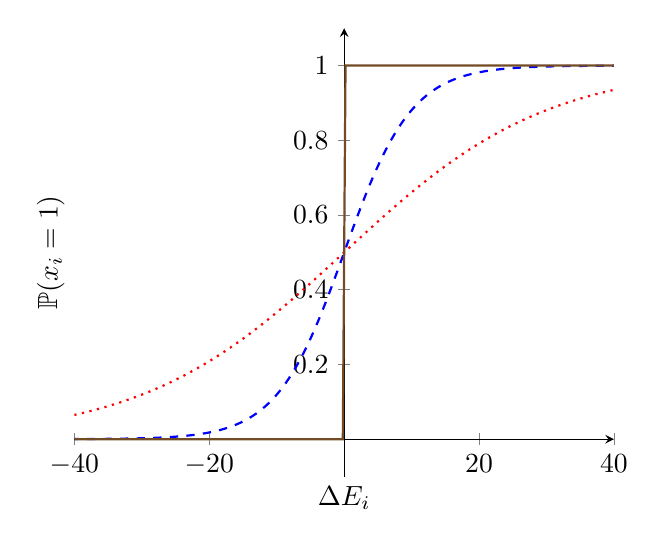
\begin{tikzpicture}
    \begin{axis}[
        domain=-80:80,
        xmin=-40, xmax=40,
        ymin=-0.1, ymax=1.1,
        samples=400,
        axis y line=center,
        axis x line=middle,
        >=stealth,
        x label style={at={(axis description cs:0.5,0)},anchor=north},
    y label style={at={(axis description cs:0,.5)},rotate=90,anchor=south},
        xlabel = $\Delta E_i$,
        ylabel = {$\mathbb{P}(x_i=1)$}
    ]
        \addplot+[mark=none,thick,dashed,color=blue] {1/(1+e^(-x/5))};
        \addplot+[mark=none,thick,dotted] {1/(1+e^(-x/15))};
        \addplot+[mark=none,thick] {1/(1+e^(-x/0.01))};
    \end{axis}
\end{tikzpicture}
\caption{$\tau=0$ (solid), $\tau=5$ (dashed), $\tau=15$ (dotted)}
\end{figure}
\end{frame}


\begin{frame}{}
\section{McCulloch-Pitts Machines}
\end{frame}

\begin{frame}{McCulloch-Pitts Machines}
\mpm{1}{0}{1}{0}{0}{1}
\note{\scriptsize
\begin{itemize}
\item state 1 is the refractory state, the neuron just fired and is unable to fire till it recovers
\item state 0 is the armed state, the neuron just recovered and is waiting to fire
\item here we model the units with the Nossenson-Messer neuron model, which explains biological firing rates in response to external stimuli
\end{itemize}}
\end{frame}


\begin{frame}{McCulloch-Pitts Machines}
\begin{figure}[h]
\centering
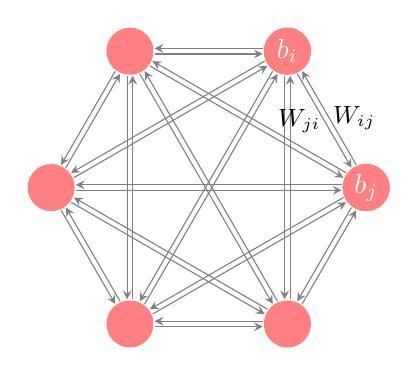
\begin{tikzpicture}[scale = 1,-,draw=black!50, node distance=\layersep,>=stealth]
    \tikzstyle{neuron}=[circle,fill=black!25,minimum size=17pt,inner sep=0pt];
    \tikzstyle{unit}=[neuron, fill=red!50,thick,];
 \def \radius {2cm}
% \def \margin {8}
 \def \n {6}
 \foreach \s in {1,...,\n}{
  \node[unit] (\s) at ({360/\n * (\s - 1) - 180}:\radius) {};
%  \node (S-\s) at ($(\s) + {360/\n * (\s - 1) - 180}:5mm$) {$s_i$};
}  

   \DoubleLine{1}{2}{<-,draw=black!50}{}{->,draw=black!50}{};
   \DoubleLine{1}{3}{<-,draw=black!50}{}{->,draw=black!50}{};
   \DoubleLine{1}{4}{<-,draw=black!50}{}{->,draw=black!50}{};
   \DoubleLine{1}{5}{<-,draw=black!50}{}{->,draw=black!50}{};
   \DoubleLine{1}{6}{<-,draw=black!50}{}{->,draw=black!50}{};
    \DoubleLine{2}{3}{<-,draw=black!50}{}{->,draw=black!50}{};
   \DoubleLine{2}{4}{<-,draw=black!50}{}{->,draw=black!50}{};
   \DoubleLine{2}{5}{<-,draw=black!50}{}{->,draw=black!50}{};
   \DoubleLine{2}{6}{<-,draw=black!50}{}{->,draw=black!50}{};
   \DoubleLine{3}{4}{<-,draw=black!50}{}{->,draw=black!50}{};
   \DoubleLine{3}{5}{<-,draw=black!50}{}{->,draw=black!50}{};
   \DoubleLine{3}{6}{<-,draw=black!50}{}{->,draw=black!50}{};
    \DoubleLine{4}{5}{<-,draw=black!50}{\small$W_{ji}$}{->,draw=black!50}{\small$W_{ij}$};
   \DoubleLine{4}{6}{<-,draw=black!50}{}{->,draw=black!50}{};
   \DoubleLine{5}{6}{<-,draw=black!50}{}{->,draw=black!50}{};

   \node[unit](i) at ({60 }:\radius) {{\color{white}$b_i$}};
   \node[unit](j) at ({360}:\radius) {{\color{white}$b_j$}};
%   \draw[color=None] (i) edge node[right] {\small $W_{ij}$} (j);
%   \draw[color=None] (i) edge node[left] {\small $W_{ij}$} (j);
\end{tikzpicture}
\end{figure}
\begin{align*}
\text{Transition Energy, }E(y,x|\theta) &= -\sum_{ji \in E}W_{ji}y_jx_i- \sum_{j \in V}b_j s_j- \sum_{i \in V}b_i s_i\\
\Gamma_{yx} &=\exp\left(-\frac{1}{2\tau}E(y,x|\theta)+\frac{1}{2\tau}E(x,x|\theta)\right)\\
\end{align*}
\note{
\scriptsize
\begin{itemize}
\item digraph, $G=(V,E)$, weights $W: V \to \mathbb{R}$, biases $b:E \to \mathbb{R}$, binary states $\mathbb{B}=\{0,1\}$ with an initial distribution $\mathbb{B}^{|V|} \to \delta$ and a temperature $\tau$
\item allow transitions where $y$ and $x$ differ by only one bit
\item here the $W$ matrix need not be symmetrical with zero diagonals like what we had in the Hopfield network and Boltzmann machine models
\item for each $y \neq x$, start a Poisson process with rate $\Gamma_{yx}$
\item as such, we can talk about the interarrival timings of the Poisson process and our simulation of the McCulloch-Pitts machine not only gives us a binary tuple, but also the time taken from it to transit from its earlier state
 \end{itemize}
}

\end{frame}

\begin{frame}{McCulloch-Pitts Machines}
\begin{figure}[h]
\centering
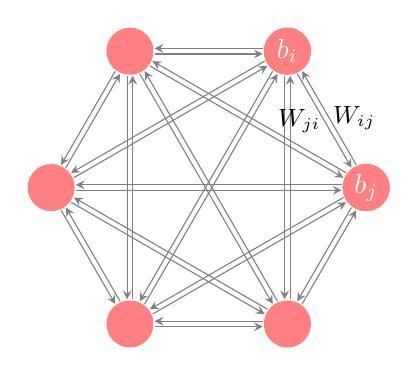
\begin{tikzpicture}[scale = 1,-,draw=black!50, node distance=\layersep,>=stealth]
    \tikzstyle{neuron}=[circle,fill=black!25,minimum size=17pt,inner sep=0pt];
    \tikzstyle{unit}=[neuron, fill=red!50,thick,];
 \def \radius {2cm}
% \def \margin {8}
 \def \n {6}
 \foreach \s in {1,...,\n}{
  \node[unit] (\s) at ({360/\n * (\s - 1) - 180}:\radius) {};
%  \node (S-\s) at ($(\s) + {360/\n * (\s - 1) - 180}:5mm$) {$s_i$};
}  

   \DoubleLine{1}{2}{<-,draw=black!50}{}{->,draw=black!50}{};
   \DoubleLine{1}{3}{<-,draw=black!50}{}{->,draw=black!50}{};
   \DoubleLine{1}{4}{<-,draw=black!50}{}{->,draw=black!50}{};
   \DoubleLine{1}{5}{<-,draw=black!50}{}{->,draw=black!50}{};
   \DoubleLine{1}{6}{<-,draw=black!50}{}{->,draw=black!50}{};
    \DoubleLine{2}{3}{<-,draw=black!50}{}{->,draw=black!50}{};
   \DoubleLine{2}{4}{<-,draw=black!50}{}{->,draw=black!50}{};
   \DoubleLine{2}{5}{<-,draw=black!50}{}{->,draw=black!50}{};
   \DoubleLine{2}{6}{<-,draw=black!50}{}{->,draw=black!50}{};
   \DoubleLine{3}{4}{<-,draw=black!50}{}{->,draw=black!50}{};
   \DoubleLine{3}{5}{<-,draw=black!50}{}{->,draw=black!50}{};
   \DoubleLine{3}{6}{<-,draw=black!50}{}{->,draw=black!50}{};
    \DoubleLine{4}{5}{<-,draw=black!50}{\small$W_{ji}$}{->,draw=black!50}{\small$W_{ij}$};
   \DoubleLine{4}{6}{<-,draw=black!50}{}{->,draw=black!50}{};
   \DoubleLine{5}{6}{<-,draw=black!50}{}{->,draw=black!50}{};

   \node[unit](i) at ({60 }:\radius) {{\color{white}$b_i$}};
   \node[unit](j) at ({360}:\radius) {{\color{white}$b_j$}};
%   \draw[color=None] (i) edge node[right] {\small $W_{ij}$} (j);
%   \draw[color=None] (i) edge node[left] {\small $W_{ij}$} (j);
\end{tikzpicture}
\end{figure}
\begin{align*}
\text{Transition Energy, }E(y,x|\theta) &= -\sum_{ji \in E}W_{ji}y_jx_i- \sum_{j \in V}b_j s_j- \sum_{i \in V}b_i s_i\\
\Gamma_{yx} &:=\exp\left(\frac{1}{2\tau}s_jz_j\right)\\
\end{align*}
where $s_j = 1-2x_j$, $z_j = \sum_{j}W_{ji}x_i + b_j$ and $x,y$ differ by the $j$th unit.

\end{frame}

\note{
\scriptsize
\begin{itemize}
\item when doing the updates we can just update the linear responses $z_j$ and apply softmax on the $\lambda_j$'s to get the probability distribution of the transitions.
\item it seems counter-intuitive to think of 0 as armed and 1 as refractory, but it is in fact the most natural thinking
\item a transition from $0 \to 1$ is a act of firing and a transition from $1 \to 0$ is the act of recovery
\item when a neuron transit from $0 \to 1$, it changes the value of the linear response; for a transiting neuron $i$, if $W_{ji}>0$, then such a transition increases the linear response of neuron $j$ and if $W_{ji}<0$ it decreases the linear response of neuron $j$
\item the sign $s$ depends on the state of the neuron, it preserves the sign of the linear response if it is armed and flips the sign of the linear response if it is refractory
 \end{itemize}
}


\begin{frame}{McCulloch-Pitts Machines}
\begin{figure}[h]
\centering
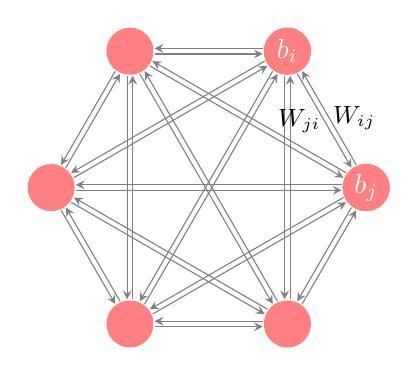
\begin{tikzpicture}[scale = 1,-,draw=black!50, node distance=\layersep,>=stealth]
    \tikzstyle{neuron}=[circle,fill=black!25,minimum size=17pt,inner sep=0pt];
    \tikzstyle{unit}=[neuron, fill=red!50,thick,];
 \def \radius {2cm}
% \def \margin {8}
 \def \n {6}
 \foreach \s in {1,...,\n}{
  \node[unit] (\s) at ({360/\n * (\s - 1) - 180}:\radius) {};
%  \node (S-\s) at ($(\s) + {360/\n * (\s - 1) - 180}:5mm$) {$s_i$};
}  

   \DoubleLine{1}{2}{<-,draw=black!50}{}{->,draw=black!50}{};
   \DoubleLine{1}{3}{<-,draw=black!50}{}{->,draw=black!50}{};
   \DoubleLine{1}{4}{<-,draw=black!50}{}{->,draw=black!50}{};
   \DoubleLine{1}{5}{<-,draw=black!50}{}{->,draw=black!50}{};
   \DoubleLine{1}{6}{<-,draw=black!50}{}{->,draw=black!50}{};
    \DoubleLine{2}{3}{<-,draw=black!50}{}{->,draw=black!50}{};
   \DoubleLine{2}{4}{<-,draw=black!50}{}{->,draw=black!50}{};
   \DoubleLine{2}{5}{<-,draw=black!50}{}{->,draw=black!50}{};
   \DoubleLine{2}{6}{<-,draw=black!50}{}{->,draw=black!50}{};
   \DoubleLine{3}{4}{<-,draw=black!50}{}{->,draw=black!50}{};
   \DoubleLine{3}{5}{<-,draw=black!50}{}{->,draw=black!50}{};
   \DoubleLine{3}{6}{<-,draw=black!50}{}{->,draw=black!50}{};
    \DoubleLine{4}{5}{<-,draw=black!50}{\small$W_{ji}$}{->,draw=black!50}{\small$W_{ij}$};
   \DoubleLine{4}{6}{<-,draw=black!50}{}{->,draw=black!50}{};
   \DoubleLine{5}{6}{<-,draw=black!50}{}{->,draw=black!50}{};

   \node[unit](i) at ({60 }:\radius) {{\color{white}$b_i$}};
   \node[unit](j) at ({360}:\radius) {{\color{white}$b_j$}};
%   \draw[color=None] (i) edge node[right] {\small $W_{ij}$} (j);
%   \draw[color=None] (i) edge node[left] {\small $W_{ij}$} (j);
\end{tikzpicture}
\end{figure}
\begin{align*}
\text{Transition probability from $x$ to $y$, }p_{yx} = \frac{\lambda_j}{\sum_{j'}\lambda_{j'}}
\end{align*}
\note{
\scriptsize
\begin{itemize}
\item when doing the updates we can just update the linear responses $z_j$ and apply softmax on the $\lambda_j$'s to get the probability distribution of the transitions.
 \end{itemize}
}

\end{frame}

%spiking starts here


\begin{frame}{McCulloch-Pitts Machines}
\mpm{1}{0}{0}{0}{1}{1}
\end{frame}

\begin{frame}{McCulloch-Pitts Machines}
\begin{figure}[h]
\centering
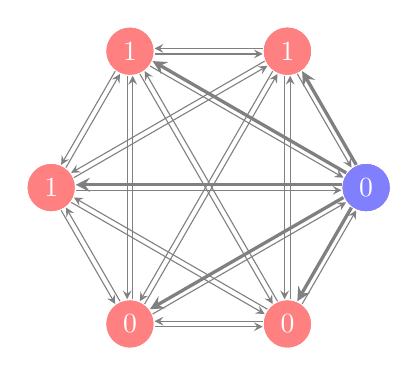
\begin{tikzpicture}[scale = 1,-,draw=black!50, node distance=\layersep,>=stealth]
    \tikzstyle{neuron}=[circle,fill=black!25,minimum size=17pt,inner sep=0pt];
    \tikzstyle{unit}=[neuron, fill=red!50,thick,];
        \tikzstyle{spike}=[neuron, fill=blue!50];

 \def \radius {2cm}
% \def \margin {8}
 \def \n {6}
 \foreach \s in {1,...,\n}{
  \node[unit] (\s) at ({360/\n * (\s - 1) - 180}:\radius) {};
%  \node (S-\s) at ($(\s) + {360/\n * (\s - 1) - 180}:5mm$) {$s_i$};
}  

   \DoubleLine{1}{2}{<-,draw=black!50}{}{->,draw=black!50}{};
   \DoubleLine{1}{3}{<-,draw=black!50}{}{->,draw=black!50}{};
   \DoubleLine{1}{4}{<-,draw=black!50,very thick}{}{->,draw=black!50}{};
   \DoubleLine{1}{5}{<-,draw=black!50}{}{->,draw=black!50}{};
   \DoubleLine{1}{6}{<-,draw=black!50}{}{->,draw=black!50}{};
    \DoubleLine{2}{3}{<-,draw=black!50}{}{->,draw=black!50}{};
   \DoubleLine{2}{4}{<-,draw=black!50,very thick}{}{->,draw=black!50}{};
   \DoubleLine{2}{5}{<-,draw=black!50}{}{->,draw=black!50}{};
   \DoubleLine{2}{6}{<-,draw=black!50}{}{->,draw=black!50}{};
   \DoubleLine{3}{4}{<-,draw=black!50,very thick}{}{->,draw=black!50}{};
   \DoubleLine{3}{5}{<-,draw=black!50}{}{->,draw=black!50}{};
   \DoubleLine{3}{6}{<-,draw=black!50}{}{->,draw=black!50}{};
    \DoubleLine{4}{5}{<-,draw=black!50}{}{->,draw=black!50,very thick}{};
   \DoubleLine{4}{6}{<-,draw=black!50}{}{->,draw=black!50,very thick}{};
   \DoubleLine{5}{6}{<-,draw=black!50}{}{->,draw=black!50}{};

   \node[unit](i) at ({60 }:\radius) {{\color{white}$b_i$}};
   \node[spike](j) at ({360}:\radius) {{\color{white}$b_j$}};
   \node[unit] (1) at (- 180:\radius) {{\color{white}1}};
   \node[unit] (2) at (- 120:\radius) {{\color{white}0}};
     \node[unit] (3) at (- 60:\radius) {{\color{white}0}};
   \node[spike] (4) at (0:\radius) {{\color{white}0}};
  \node[unit] (5) at (60:\radius) {{\color{white}1}};
   \node[unit] (6) at (120:\radius) {{\color{white}1}};
%   \draw[color=None] (i) edge node[right] {\small $W_{ij}$} (j);
%   \draw[color=None] (i) edge node[left] {\small $W_{ij}$} (j);
\end{tikzpicture}
\end{figure}
\begin{align*}
\left(T_0,(1,0,0,0,1,1)\right)
\end{align*}

%\begin{align*}
%\text{Transition Energy, }E(y,x|\theta) &= -\sum_{ji \in E}W_{ji}y_jx_i- \sum_{j \in V}b_j s_j- \sum_{i \in V}b_i s_i\\
%\Gamma_{yx} &=\exp\left(-\frac{1}{2\tau}E(y,x|\theta)+\frac{1}{2\tau}E(x,x|\theta)\right)\\
%\end{align*}
%where $G=(V,E)$ digraph, $\theta = (W, b, \tau)$
\end{frame}


\begin{frame}{McCulloch-Pitts Machines}
\begin{figure}[h]
\centering
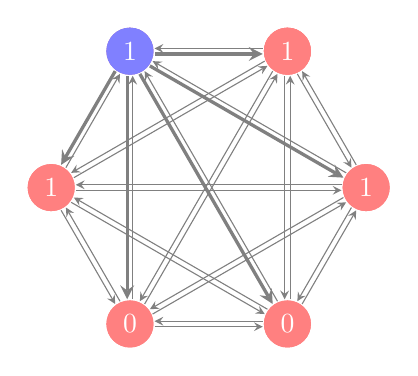
\begin{tikzpicture}[scale = 1,-,draw=black!50, node distance=\layersep,>=stealth]
    \tikzstyle{neuron}=[circle,fill=black!25,minimum size=17pt,inner sep=0pt];
    \tikzstyle{unit}=[neuron, fill=red!50,thick,];
        \tikzstyle{spike}=[neuron, fill=blue!50];

 \def \radius {2cm}
% \def \margin {8}
 \def \n {6}
 \foreach \s in {1,...,\n}{
  \node[unit] (\s) at ({360/\n * (\s - 1) - 180}:\radius) {};
%  \node (S-\s) at ($(\s) + {360/\n * (\s - 1) - 180}:5mm$) {$s_i$};
}  

   \DoubleLine{1}{2}{<-,draw=black!50}{}{->,draw=black!50}{};
   \DoubleLine{1}{3}{<-,draw=black!50}{}{->,draw=black!50}{};
   \DoubleLine{1}{4}{<-,draw=black!50}{}{->,draw=black!50}{};
   \DoubleLine{1}{5}{<-,draw=black!50}{}{->,draw=black!50}{};
   \DoubleLine{1}{6}{<-,draw=black!50,very thick}{}{->,draw=black!50}{};
    \DoubleLine{2}{3}{<-,draw=black!50}{}{->,draw=black!50}{};
   \DoubleLine{2}{4}{<-,draw=black!50}{}{->,draw=black!50}{};
   \DoubleLine{2}{5}{<-,draw=black!50}{}{->,draw=black!50}{};
   \DoubleLine{2}{6}{<-,draw=black!50,very thick}{}{->,draw=black!50}{};
   \DoubleLine{3}{4}{<-,draw=black!50}{}{->,draw=black!50}{};
   \DoubleLine{3}{5}{<-,draw=black!50}{}{->,draw=black!50}{};
   \DoubleLine{3}{6}{<-,draw=black!50,very thick}{}{->,draw=black!50}{};
    \DoubleLine{4}{5}{<-,draw=black!50}{}{->,draw=black!50}{};
   \DoubleLine{4}{6}{<-,draw=black!50,very thick}{}{->,draw=black!50}{};
   \DoubleLine{5}{6}{<-,draw=black!50,very thick}{}{->,draw=black!50}{};

   \node[unit](i) at ({60 }:\radius) {{\color{white}$b_i$}};
   \node[spike](j) at ({120}:\radius) {{\color{white}$b_j$}};
   \node[unit] (1) at (- 180:\radius) {{\color{white}1}};
   \node[unit] (2) at (- 120:\radius) {{\color{white}0}};
     \node[unit] (3) at (- 60:\radius) {{\color{white}0}};
   \node[unit] (4) at (0:\radius) {{\color{white}1}};
  \node[unit] (5) at (60:\radius) {{\color{white}1}};
   \node[spike] (6) at (120:\radius) {{\color{white}1}};
%   \draw[color=None] (i) edge node[right] {\small $W_{ij}$} (j);
%   \draw[color=None] (i) edge node[left] {\small $W_{ij}$} (j);
\end{tikzpicture}
\end{figure}
\begin{align*}
\left(T_0,(1,0,0,0,1,1)\right)\\
\left(T_1,(1,0,0,1,1,1)\right)
\end{align*}

%\begin{align*}
%\text{Transition Energy, }E(y,x|\theta) &= -\sum_{ji \in E}W_{ji}y_jx_i- \sum_{j \in V}b_j s_j- \sum_{i \in V}b_i s_i\\
%\Gamma_{yx} &=\exp\left(-\frac{1}{2\tau}E(y,x|\theta)+\frac{1}{2\tau}E(x,x|\theta)\right)\\
%\end{align*}
%where $G=(V,E)$ digraph, $\theta = (W, b, \tau)$
\end{frame}

\begin{frame}{McCulloch-Pitts Machines}
\begin{figure}[h]
\centering
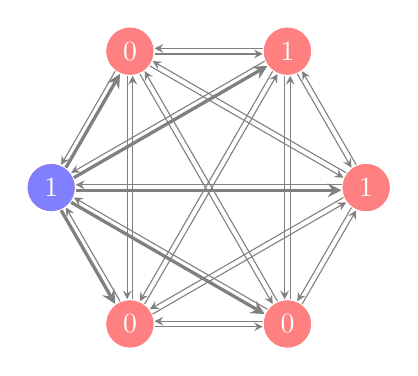
\begin{tikzpicture}[scale = 1,-,draw=black!50, node distance=\layersep,>=stealth]
    \tikzstyle{neuron}=[circle,fill=black!25,minimum size=17pt,inner sep=0pt];
    \tikzstyle{unit}=[neuron, fill=red!50,thick,];
        \tikzstyle{spike}=[neuron, fill=blue!50];

 \def \radius {2cm}
% \def \margin {8}
 \def \n {6}
 \foreach \s in {1,...,\n}{
  \node[unit] (\s) at ({360/\n * (\s - 1) - 180}:\radius) {};
%  \node (S-\s) at ($(\s) + {360/\n * (\s - 1) - 180}:5mm$) {$s_i$};
}  

   \DoubleLine{1}{2}{<-,draw=black!50}{}{->,draw=black!50,very thick}{};
   \DoubleLine{1}{3}{<-,draw=black!50}{}{->,draw=black!50,very thick}{};
   \DoubleLine{1}{4}{<-,draw=black!50}{}{->,draw=black!50,very thick}{};
   \DoubleLine{1}{5}{<-,draw=black!50}{}{->,draw=black!50,very thick}{};
   \DoubleLine{1}{6}{<-,draw=black!50}{}{->,draw=black!50,very thick}{};
    \DoubleLine{2}{3}{<-,draw=black!50}{}{->,draw=black!50}{};
   \DoubleLine{2}{4}{<-,draw=black!50}{}{->,draw=black!50}{};
   \DoubleLine{2}{5}{<-,draw=black!50}{}{->,draw=black!50}{};
   \DoubleLine{2}{6}{<-,draw=black!50}{}{->,draw=black!50}{};
   \DoubleLine{3}{4}{<-,draw=black!50}{}{->,draw=black!50}{};
   \DoubleLine{3}{5}{<-,draw=black!50}{}{->,draw=black!50}{};
   \DoubleLine{3}{6}{<-,draw=black!50}{}{->,draw=black!50}{};
    \DoubleLine{4}{5}{<-,draw=black!50}{}{->,draw=black!50}{};
   \DoubleLine{4}{6}{<-,draw=black!50}{}{->,draw=black!50}{};
   \DoubleLine{5}{6}{<-,draw=black!50}{}{->,draw=black!50}{};

   \node[spike] (1) at (- 180:\radius) {{\color{white}1}};
   \node[unit] (2) at (- 120:\radius) {{\color{white}0}};
     \node[unit] (3) at (- 60:\radius) {{\color{white}0}};
   \node[unit] (4) at (0:\radius) {{\color{white}1}};
  \node[unit] (5) at (60:\radius) {{\color{white}1}};
   \node[unit] (6) at (120:\radius) {{\color{white}0}};
%   \draw[color=None] (i) edge node[right] {\small $W_{ij}$} (j);
%   \draw[color=None] (i) edge node[left] {\small $W_{ij}$} (j);
\end{tikzpicture}
\end{figure}
\begin{align*}
\left(T_0,(1,0,0,0,1,1)\right)\\
\left(T_1,(1,0,0,1,1,1)\right)\\
\left(T_2,(1,0,0,1,1,0)\right)
\end{align*}

%\begin{align*}
%\text{Transition Energy, }E(y,x|\theta) &= -\sum_{ji \in E}W_{ji}y_jx_i- \sum_{j \in V}b_j s_j- \sum_{i \in V}b_i s_i\\
%\Gamma_{yx} &=\exp\left(-\frac{1}{2\tau}E(y,x|\theta)+\frac{1}{2\tau}E(x,x|\theta)\right)\\
%\end{align*}
%where $G=(V,E)$ digraph, $\theta = (W, b, \tau)$
\end{frame}

%spiking ends here


\begin{frame}{McCulloch-Pitts Machines}

\end{frame}

\begin{frame}{McCulloch-Pitts Machines}

\end{frame}

\begin{frame}{}
\section{Simulating on GPUs}
\end{frame}

\begin{frame}{Simulating on GPUs}
\begin{figure}[h]
  \centering
  \tikzstyle{trans-name}=[anchor=north west]
  \tikzstyle{alu}=[fill=green!80!black!30]
  \tikzstyle{data}=[fill=orange!50]
  \tikzstyle{ctrl}=[fill	=red!40]
  \subfigure[CPU] {
    \begin{tikzpicture}[scale=0.8]
      \draw[ctrl] (0, 6)   rectangle +(3, -2);
      \draw[data] (0, 4)   rectangle +(6, -2);
      \draw[data] (0, 1.5) rectangle +(6, -1);
      \node[trans-name] at (0, 6) {Control};
      \node[trans-name] at (0, 4) {Cache};
      \node[trans-name] at (0, 1.5) {DRAM};
      \foreach \x in {3, 4.5}
        \foreach \y in {5, 6} {
          \draw[alu] (\x, \y) rectangle +(1.5, -1);
          \node[trans-name] at (\x, \y) {ALU};
        }
    \end{tikzpicture}
  }
  \subfigure[GPU] {
    \begin{tikzpicture}[scale=0.8]
      \draw[data] (0, 1.5) rectangle +(6, -1);
      \node[trans-name] at (0, 1.5) {DRAM};
      \foreach \x in {0.5, 1, ..., 5.5}
        \foreach \y in {2.5, 3, ..., 6}
          \draw[alu] (\x, \y) rectangle +(0.5, -0.46);
      \foreach \y in {2.5, 3, ..., 6}
        \draw[ctrl] (0, \y) rectangle +(0.5, -0.23);
      \foreach \y in {2.27, 2.77, ..., 6}
        \draw[data] (0, \y) rectangle +(0.5, -0.23);
    \end{tikzpicture}
  }
  \caption[Comparison between CPU and GPU layout]{
    Comparison between the amount of transistors
    devoted to different functions inside a CPU and a GPU.
    %Arithmetic logic units (ALUs) perform data processing.
%    (This picture is copied from~\cite[\S1]{cudaprog2}).
  }
\end{figure}
\end{frame}


\begin{frame}{Simulating on GPUs}


\begin{figure}[h]
  \centering
  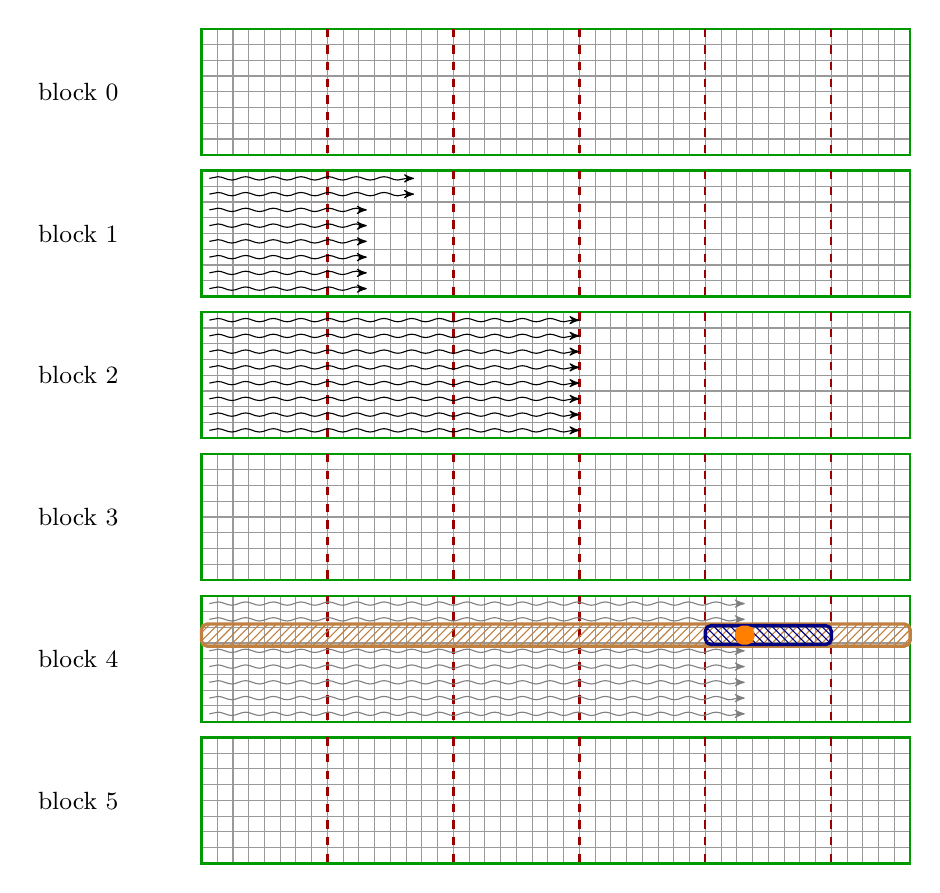
\begin{tikzpicture}[scale=.2, yscale=-1, font=\small]

    \def\nrbodies{45}     \def\lastbody{44}
    \def\nrblocks{6}      \def\lastblock{5}
    \def\nrtiles{6}       \def\lasttile{5}
    \def\nrblockbodies{8} \def\lastblockbody{7}

    \foreach \block in {0,1,...,\lastblock} {
      %\def\ybot{9 * \block}
      \pgfmathsetmacro{\ybot}{(1 + \nrblockbodies) * \block}
      \draw[innergrid] (0, \ybot) grid      ++(\nrbodies, \nrblockbodies);
      \draw[tile]      (0, \ybot) rectangle ++(\nrbodies, \nrblockbodies);
      %\draw (1 + \nrbodies, \ybot + \nrblockbodies / 2)
      \draw (-11, \ybot + \nrblockbodies / 2)
          node[anchor=west] { block $\block$ };

      \foreach \syncpoint in {1,...,\lasttile}
        \draw[sync] (\nrblockbodies * \syncpoint, \ybot) -- ++(0, \nrblockbodies);
    }

    %\def\block{2}
   %\foreach \k in {0,...,3}
    %  \drawthread{thread}{\block}{\k}{43};
    %\foreach \k in {4,...,\lastblockbody}
    %  \drawthread{thread}{\block}{\k}{42};

    \def\block{1}
    \foreach \k in {0,1}
      \drawthread{thread}{\block}{\k}{14};
    \foreach \k in {2,...,\lastblockbody}
      \drawthread{thread}{\block}{\k}{11};

    \def\block{2}
    \foreach \k in {0,...,\lastblockbody}
      \drawthread{thread}{\block}{\k}{24.5};

    \def\block{4}
    \def\to{35}
    \foreach \k in {0,1,3,4,...,\lastblockbody}
      \drawthread{thread, gray}{\block}{\k}{\to};

    % draw kernel calls
    \def\currentx{34}
    \pgfmathsetmacro{\tilestart}{floor(\currentx / \nrblockbodies) * \nrblockbodies}
    \pgfmathsetmacro{\ybot}{(\nrblockbodies + 1) * \block}
    \def\currenty{\ybot + 2}
    \draw[kernelcall=brown, pattern=north east lines]
      (   0, \currenty - .2) rectangle ++(\nrbodies, 1.4);
    \draw[kernelcall=blue!50!black, pattern=north west lines]
      (\tilestart, \currenty - .1) rectangle ++(\nrblockbodies, 1.2);
    \draw[kernelcall=orange, fill]
      (\currentx, \currenty) rectangle ++( 1, 1);
    \node[anchor=base] (interactionanchor) at (\currentx + 0.5, \currenty + 1.0) {};
    \node[anchor=base] (tileanchor)        at (\currentx + 2.5, \currenty + 1.1) {};
    \node[anchor=base] (evalanchor)        at (\currentx - 8.5, \currenty + 1.2) {};
%
%    \node[imglabel] (interactionlabel) at (49.5, \currenty +  4.5) {\verb!particle_interaction!};
%    \node[imglabel] (tilelabel)        at (49.5, \currenty +  7.5) {\verb!update_tile!};
%    \node[imglabel] (evallabel)        at (49.5, \currenty + 10.5) {\verb!eval_derivatives!};
%
%    \draw[kernelarrow, orange]        (interactionanchor.base) to (interactionlabel);
%    \draw[kernelarrow, blue!50!black] (tileanchor.base)        to (tilelabel);
%    \draw[kernelarrow, brown]         (evalanchor.base)        to (evallabel);
%
%    \drawthread{thread}{\block}{2}{\to};
%
%    \def\examplex{21}
%    \def\exampley{5}
%    \draw[examplecell] (\examplex, \exampley) rectangle ++(1, 1);
%    \node[anchor=base] (cellanchor) at (\examplex + .5, \exampley + .5) {};
%
%    \draw (35, -4) node[imglabel, anchor=west] (interaction) {
%      \(
%       \left\{
%       \begin{aligned}
%         {\vec U}_{pq} &= α_q\,\K_ε(\x_p - \x_q) \\
%         A_{pq}        &= [α_q - α_p]\,η_ε(\x_p - \x_q) \\
%       \end{aligned}
%       \right.
%      \)
%    };
%    \draw[->, out=-45, in=180] (cellanchor.base) to (interaction);
%    \node[imglabel, anchor=east]  (plabel) at (\examplex - 7,  \exampley + .5) {\((x_p, y_p, α_p)\)};
%    \node[imglabel, anchor=south] (qlabel) at (\examplex + .5, -1) {\((x_q, y_q, α_q)\)};
%    \draw[dotted, very thick] (plabel) -- (cellanchor.base);
%    \draw[dotted, very thick] (qlabel) -- (cellanchor.base);
%
%    \foreach \block in {1,2,4} {
%      \pgfmathsetmacro{\ybot}{(1 + \nrblockbodies) * \block}
%      \foreach \thread in {0,...,\lastblockbody} {
%        \node[font=\tiny, anchor=east] at (0, .5 + \ybot + \thread) {\thread};
%      }
%    }
%
%    \def\nridlethreads{3}
%    \fill[pattern=north east lines] (0, 50) rectangle ++(\nrbodies, 3);
%    \node[imglabel, anchor=center] (idlelabel) at (\nrbodies / 2, 51.5) {idle threads};

  \end{tikzpicture}
\end{figure}
\end{frame}


\begin{frame}{Simulating on GPUs}

\end{frame}



\begin{frame}
\frametitle{References}
\begin{thebibliography}{}
\bibitem[Macor, 2015]{Macor}
J. ~Macor.
\newblock {\em A Brief Introduction to Type Theory and the Univalence Axiom}
\newblock \href{http://math.uchicago.edu/~may/REU2015/REUPapers/Macor.pdf}{\footnotesize http://math.uchicago.edu/~may/REU2015/REUPapers/Macor.pdf}


\bibitem[UFP, 2013]{hottbook}
The {Univalent Foundations Program}
\newblock {\em Homotopy Type Theory: Univalent Foundations of Mathematics}.
\newblock \href{https://homotopytypetheory.org/book}{\footnotesize https://homotopytypetheory.org/book}

\bibitem[Caf$\acute{\text{e}}$, 2013]{settotype}
    The n-Category Caf$\acute{\text{e}}$
\newblock {\em From Set Theory to Type Theory}
\newblock \href{https://golem.ph.utexas.edu/category/2013/01/from_set_theory_to_type_theory.html}{\footnotesize https://golem.ph.utexas.edu/category/2013/01/from\_set\_theory\_to\_type\_theory.html}

\bibitem[ncatlab, 2015]{nlab}
The $n$Lab
\newblock {\em Function Type}
\newblock \href{https://ncatlab.org/nlab/show/function+type}{\footnotesize https://ncatlab.org/nlab/show/function+type}

\end{thebibliography}
\end{frame}

\end{document}

